\documentclass{standalone}
\usepackage{tikz}
\usepackage{adjustbox}
\usepackage{helvet}  
\usepackage{sansmathfonts}  
\renewcommand{\familydefault}{\sfdefault}  
\usetikzlibrary{arrows.meta,calc,decorations.pathmorphing}
\usetikzlibrary{shapes.geometric, shapes.arrows}
\usepackage{xcolor}

\definecolor{color0000FF}{HTML}{0000FF}
\definecolor{color91A9CE}{HTML}{91A9CE}
\definecolor{color00FF00}{HTML}{00FF00}
\definecolor{color90EE90}{HTML}{90EE90}
\definecolor{colorFF00FF}{HTML}{FF00FF}
\definecolor{colorFFB6C1}{HTML}{FFB6C1}
\begin{document}
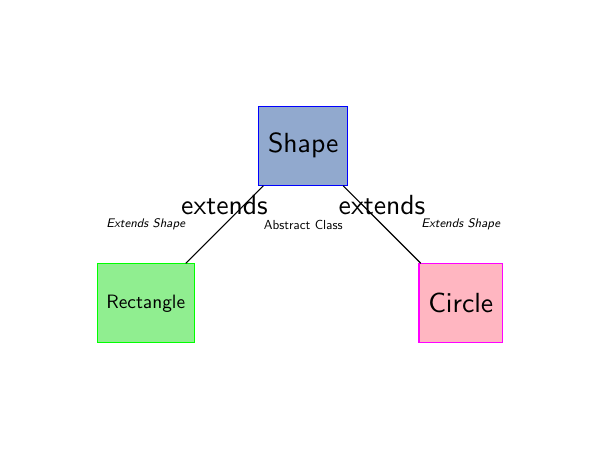
\begin{tikzpicture}
\useasboundingbox (-3.5,-1.5) rectangle (3.5,3.5);



\node[draw=color0000FF, fill=color91A9CE, minimum width=1cm, minimum height=1cm] (shape) at (0,2) {\adjustbox{max width=1cm, max height=1cm}{Shape}};
\node[draw=color00FF00, fill=color90EE90, minimum width=1cm, minimum height=1cm] (rectangle) at (-2,0) {\adjustbox{max width=1cm, max height=1cm}{Rectangle}};
\node[draw=colorFF00FF, fill=colorFFB6C1, minimum width=1cm, minimum height=1cm] (circle) at (2,0) {\adjustbox{max width=1cm, max height=1cm}{Circle}};
\node[draw=none, minimum width=1cm, minimum height=1cm] (shape_label) at (0,1) {\adjustbox{max width=1cm, max height=1cm}{Abstract Class}};
\node[draw=none, font=\small\it, minimum width=1cm, minimum height=1cm] (rectangle_label) at (-2,1) {\adjustbox{max width=1cm, max height=1cm}{Extends Shape}};
\node[draw=none, font=\small\it, minimum width=1cm, minimum height=1cm] (circle_label) at (2,1) {\adjustbox{max width=1cm, max height=1cm}{Extends Shape}};
\draw[] (rectangle) (rectangle) to node[above] {extends} (shape);
\draw[] (circle) (circle) to node[above] {extends} (shape);

\end{tikzpicture}
\end{document}